\textsf{ANN-Benchmarks} is implemented as a Python framework with several
different interfaces: one script for running experiments and a handful of
others for
working with and plotting results. It automatically downloads datasets when
they are needed and uses Docker build files to install algorithm implementations
and their dependencies.

%The experiment front-end has some
%parameters of its own that influence what algorithm implementations will be
%tested: the dataset to be used, the number of neighbours to search for, and the distance
%metric to be used to compare points. The plotting front-ends are also aware
%of these parameters, which are used to select and label plots.

This section gives only a high-level overview of the system; see
\url{http://ann-benchmarks.com} for more detailed technical
information.

\subsection{Algorithm implementations}

Each implementation is installed via a Docker build file. These files specify
how an implementation should be installed on a standard Ubuntu system by
building and installing its dependencies and code. ANN-Benchmarks requires that
this installation process also build Python wrappers for the implementation
to give the framework access to it. 

%Each dataset and library has a shell script that downloads, builds and installs
%it. These scripts are built on top of a shell function library that defines a
%few common operations, like cloning and patching a Git repository or
%downloading a dataset and checking its integrity. Datasets may also need to be
%converted; we include Python scripts for converting a few commonly-used formats
%into the plain-text format used by our system, and the shell scripts make use
%of these.
%
%Although we hope that algorithm libraries will normally bundle their own
%Python bindings, our shell function library can also apply a patch series to
%an implementation once it has been downloaded, allowing us to (temporarily)
%carry patches for bindings that will later be moved upstream.

Adding support for a new algorithm implementation to \textsf{ANN-Benchmarks} is
as easy as
writing a Docker file to install it and its dependencies, making it available to
Python by writing a wrapper (or by reusing an existing one), and adding the
parameters to be tested to the configuration files. Most of the installation
scripts fetch the latest version of their library from its Git repository,
but there is no requirement to do this; indeed, installing several different
versions of a library would make it possible to use the framework for
regression testing.

At this point, we again emphasise that we are comparing algorithm
\emph{implementations}. Implementations make many different decisions that will
affect their performance and two implementations of the same algorithm
can have somewhat different performance characteristics \cite{KriegelSZ17}.
When implementations expose other quality measures -- such as the number of
distance computations, which are more suited for comparing algorithms on a
more abstract level -- our framework will also collect this information.

\medskip
\noindent{\textbf{Local mode.}}
Using Docker is ideal for evaluating the performance of well-tuned
implementations, but ANN-Benchmarks can also be used to help in the \emph{development} process.
To support this use case, the framework provides a \emph{local mode}, which
runs processes locally on the host system and not inside a Docker container.
This makes it much easier to build a pipeline solution to, for example,
automatically check how changes in the implementation influence its performance
-- in the standard Docker setup, each change would require the Docker container to be rebuilt.

\medskip
\noindent{\textbf{Algorithm wrappers.}}
To be usable by our system, each of the implementations to be tested
must have some kind of Python interface. Many libraries already
provide their own Python wrappers, either written by hand or automatically
generated using a tool like SWIG; others are implemented partly or entirely
in Python.

% What, though, can be done about libraries with no Python bindings? How can they
% be brought into the framework?

% \subsubsubsection{SWIG}

% Wrapper generators like SWIG are powerful, but not always easy to use,
% particularly if the generator does not completely support a feature used by
% the code. We implement a lighter-weight approach --- a simple text-based
% protocol
To bring implementations that do not provide a Python interface into the
framework,
we specify a simple text-based protocol that supports the few operations we
care about: parameter configuration,
sending training data, and running queries. The framework comes with a wrapper
that communicates with external programs using this protocol.
In this way, experiments can be run in
external front-end processes implemented in any programming language.
% (although
% we provide a simple C implementation of the front-end side of the protocol as
% well).

% A front-end begins in the configuration mode, which is used to set the
% algorithm's parameters (and to negotiate the use of special protocol features).
% Once this is complete, it moves into training mode, where each item of training
% data is parsed and given an identifier. Finally, it transitions into query
% mode, which returns the identifiers of the near neighbours of a query point;
% after this, the front-end will exit.

The protocol has been designed to be easy to implement. Every message is a line
of text that will be split into tokens according to the rules of the POSIX
shell, good implementations of which are available for most programming
languages.
% A message
% sent to the front-end is known as a ``command'', while a message sent by the
% front-end is a ``reply''; the front-end only ever generates replies in response
% to a command, so both sides can synchronise their communications simply by
% performing normal blocking I/O. Replies all begin with a special marker token,
% so there is no
% need to suppress any existing output messages. Commands can affect or query the
% state of the front-end's current mode or move to the next mode, but they
% cannot move back to a previous mode, so the protocol requires almost no
% persistent state of its own.
The protocol is flexible and extensible: front-ends are free to
include extra information in replies, and they can also implement special
configuration options that cause them to diverge from the protocol's basic
behaviour. As the framework has developed new operating modes, we have
documented and implemented extensions to the protocol that allow it to take
advantage of these modes.

The overhead imposed by using plain text representations is not entirely
negligible; our benchmarks suggest that a linear search running in a subprocess
using the protocol runs at about 75\% of the speed of the same search called
directly in the same process. On the other hand, the framework has operating
modes that
reduce this overhead virtually to zero, which we will discuss in
Section~\ref{system:mtbatch}.

Note, furthermore, that we have not been able to benchmark the overhead of
other interfaces; it is quite likely, for example, that automatically generated
wrappers, which construct many Python proxy objects to precisely mirror the
underlying system, might impose a similar cost.

\subsection{Datasets and ground truth}

By default, the framework fetches datasets on demand from a remote server.
These dataset files contain, in HDF5 format,
the set of data points,
the set of query points,
the distance metric that should be used to compare them,
a list of the true nearest $k = 100$ neighbours for each query point,
and a list of the distances of each of these neighbours from the query point.

The framework also includes a script for generating dataset files from the
original datasets. Although using the precomputed hosted versions is normally
simpler, the script can be used to, for example, build a dataset file with a
different value of $k$, or to convert a private dataset for the framework's
use.

Most of the datasets use as their query set a pseudorandomly-selected set of
ten thousand entries separated from the rest of the training data; others have
separate query sets. The dataset file generation script makes this decision.

\subsection{Creating algorithm instances}

\begin{figure}[t!]
\vspace{-2em}
\begin{lstlisting}[language=yaml]
float:
  euclidean:
    megasrch:
      docker-tag: ann-benchmarks-megasrch
      module: ann_benchmarks.algorithms.MEGASRCH
      constructor: MEGASRCH
      base-args: ["@metric"]
      run-groups:
        shallow-point-lake:
          args: ["lake", [100, 200]]
          query-args: [100, [100, 200, 400]]
        deep-point-ocean:
          args: ["sea", 1000]
          query-args: [[1000, 2000], [1000, 2000, 4000]]
\end{lstlisting}
\vspace{-2em}
\caption{An example of a fragment of an algorithm configuration file.}
\label{fig:overview:example}
\end{figure}

After loading the dataset, the framework moves on to creating the algorithm
instances. It does so based on a YAML configuration file that specifies a
hierarchy of dictionaries: the first level specifies the point type, the second
the distance metric, and the third each algorithm implementation to be tested.
Each implementation
gives the name of its wrapper's Python constructor; a number of other entries
are then expanded to give the arguments to that constructor.
Figure~\ref{fig:overview:example} shows an example of this configuration file.

The \texttt{base-args} list consists of those arguments that should be
prepended to every invocation of the constructor. Figure~\ref{fig:overview:example}
also shows one of the special keywords, \texttt{"@metric"}, that is used to
pass one of the framework's configuration parameters to the constructor.

Algorithms must specify one or more ``run groups``, each of which will be
expanded into one or more lists of constructor arguments. The \texttt{args}
entry completes the argument list, but not directly:
instead, the Cartesian product of all of its entries is used to generate
\emph{many} lists of arguments. 
Another entry, \texttt{query-args}, is expanded in the same way as \texttt{args},
but each argument list generated from it is used to reconfigure the query
parameters of an algorithm instance after its internal data structures have
been built. This allows built data structures to be reused, greatly reducing
duplicated work.

As an example,
the \texttt{megasrch} entry in 
Figure~\ref{fig:overview:example} expands into
three different algorithm instances: \texttt{MEGASRCH("euclidean", "lake", 100)},
\texttt{MEGASRCH("euclidean", "lake", 200)}, and \texttt{MEGASRCH("euclidean", "sea", 1000)}. Each of
these will be trained once and then used to run a number of experiments: the
first two will run experiments with each of the query parameter groups \texttt{[100, 100]},
\texttt{[100, 200]}, and \texttt{[100, 400]} in turn, while the last will run
its experiments with the query parameter groups
\texttt{[1000, 1000]}, \texttt{[1000, 2000]}, \texttt{[1000, 4000]},
\texttt{[2000, 1000]}, \texttt{[2000, 2000]}, and \texttt{[2000, 4000]}.


% (Some algorithm constructors take dictionaries as arguments; analogous support
% exists for these as well.)


\subsection{The experiment loop}

\begin{wrapfigure}{l}{0.5\textwidth}
\vspace{-20pt}
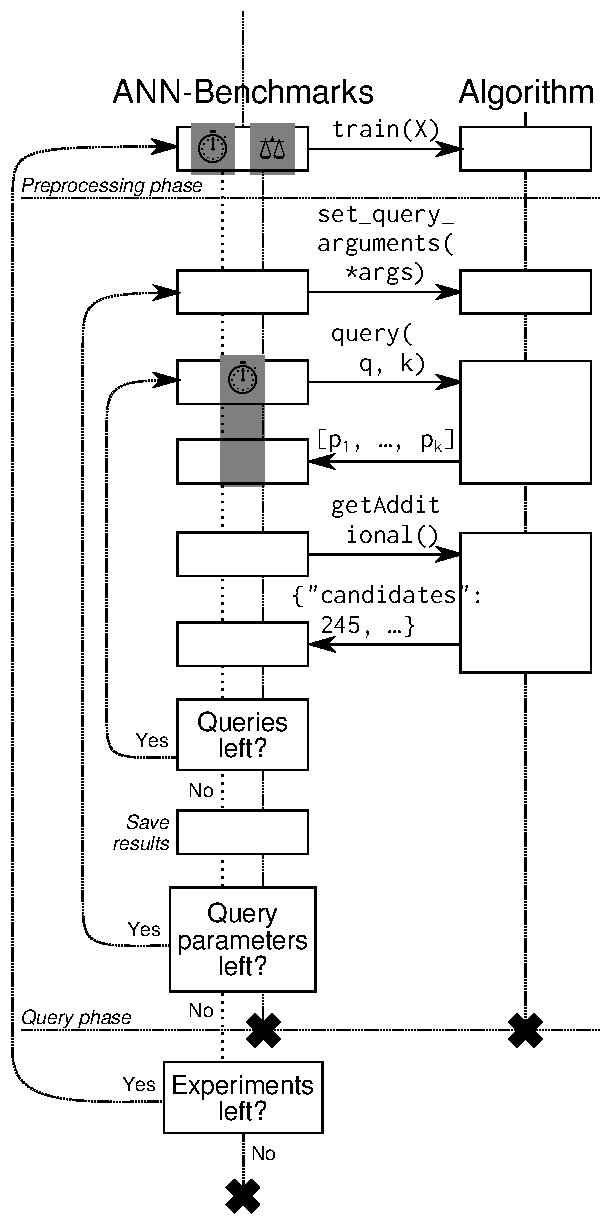
\includegraphics[width=0.5\textwidth]{scheme-v}
\caption{Overview of the interaction between ANN-Benchmarks and an algorithm
instance under test.}
\label{fig:overview:experiment}
\end{wrapfigure}

Once the framework knows what instances should be run, it moves on to the
experiment
loop, shown in Figure~\ref{fig:overview:experiment}.
The loop consists of two phases.
In the \emph{preprocessing phase}, an algorithm instance builds an index data
structure for the dataset $X$, while the framework records how long this takes
and how much additional memory it uses.
The loop then transitions to the \emph{query
phase}, in which query points are sent one by one to the algorithm instance,
while the framework records how long the responses take to arrive.
For each query point, the instance returns (at most) $k$ data points; after
answering a query, it can also report any extra
information it might have, such as the number of candidates considered, i.e., 
the number of exact distances computed. The instance
is then reconfigured with a new set of query parameters, and the query set is
run repeatedly, until no more sets of these parameters remain.

Each algorithm instance is run in an isolated Docker container. This makes it
easy to clean up after each run: simply terminating the container 
takes care of everything. Moving experiments out of the main process
also gives us an
implementation-agnostic way of computing the approximate memory usage of an
implementation:
the subprocess records its total memory consumption before and after
initialising the algorithm instance's data structures and compares the two
values. (This value is necessarily only an rough estimate -- in particular,
it cannot take into account garbage collection, or processes that use and then
attempt to release lots of temporary memory during the training process -- but
it is nevertheless useful to have.)

The complete results of each run are written to the host by mounting
part of the file system into the Docker container. The main process performs a
blocking, timed wait on the container, and will terminate it if
the user-configurable timeout is exceeded before any results are available.


\medskip

\noindent\textbf{Dataset size.} In its current form, ANN-Benchmarks
only supports
benchmarking \emph{in-memory} nearest-neighbor algorithms. In particular, the dataset is kept 
in memory by ANN-Benchmarks when running experiments. This has to be taken into account when choosing datasets to include into the framework. In practice, we need a machine with 32GB of RAM to run all the experiments, where the largest dataset has around 1\,000\,000 items consisting of 1\,000 dimensions each.

\subsection{Batched queries and multi-threading}
\label{system:mtbatch}

Running queries one by one is not necessarily representative of real-world
query workloads; many systems allow queries to be batched together.
ANN-Benchmarks has an alternative operating mode, \emph{batch mode}, in which
all the queries are passed, and all the results are returned, at once.
This enables many interesting approaches to parallelization that would not be
possible when running single queries.

When not running in batch mode, ANN-Benchmarks locks the Docker container that
hosts the experiment loop to a single thread on a single CPU, using the Linux
kernel's \texttt{cpusets} capabilities to restrict access to the system's
resources. This is intended to make comparisons fairer: without this lock,
the structure of the loop would give an implementation that ran a single
query across multiple threads an unfair advantage over an implementation
designed to use multi-threading to run several queries at once. In batch mode,
all of the host system's resources are made available to the Docker container.

The behaviour of the experiment loop diverges slightly from Figure~\ref{fig:overview:experiment} in batch mode. Batch queries do not return a sequence of tuples containing answers to the individual queries; instead, these results are obtained via an additional method, akin to Figure~\ref{fig:overview:experiment}'s \texttt{getAdditional()} method. This allows an algorithm to return the result of a batch query as an opaque internal data structure; this will stop the clock, and the additional call can then transform that data structure into Python objects without that transformation imposing a performance penalty.

Batch query mode is particularly useful when an algorithm will perform computation on the other side of a hard boundary. When using a GPU, for example, copying a single query point to its memory and then transferring the result back can be a dominating part of the query time, as we will see in Section~\ref{sec:evaluation}.
Similarly, algorithms that use the text-based protocol to communicate with a subprocess benefit enormously from batch query mode; allowing the framework to discount the overhead of string parsing and unparsing reduces the overhead virtually to zero.

\subsection{Results and metrics}

% is a
% little unusual. The mlpack benchmarking system does not do this, instead
% recording only the metrics reported by each algorithm;
% \matodo{What does SatEx do?}

For each run, we store the full name -- including the parameters -- of the
algorithm instance, the time it took to build its index data structure, and the
results of every query: the near neighbours returned by the algorithm, the time
it took to find these, and their distances from the query point, along with any
additional information the implementation might have exposed.
(To avoid affecting the timing of algorithms that do not indicate
the distance of a result, the experiment loop independently re-computes
distance values after the query has otherwise finished.)

The results of each run are stored in a separate HDF5 file in a directory
hierarchy that encodes
part of the framework's configuration. % (This is an implementation detail; the
% experiment loop simply passes the results and the configuration to a function
% that makes this decision, and the plotting scripts use enumeration functions
% that conceal the underlying structure.)
Keeping runs in separate files makes them easy to enumerate and easy to re-run,
and individual
results -- or sets of results -- can easily be shared to make results more
transparent.

Metric functions are passed the ground truth and the results for a particular
run; they can then compute their result however they see fit. Adding a new
quality metric is a matter of writing a short Python function and adding it to
an internal data structure; the plotting scripts query this data structure and
will automatically support the new metric.

\subsection{Frontend}\label{sec:frontend}

\textsf{ANN-Benchmarks} provides two options to evaluate the results of the experiments: a script to generate individual plots using Python's \textsf{matplotlib}, and another to generate a website that summarizes the results and provides interactive plots with the option to export the plot as {\LaTeX} code using \textsf{pgfplots}. See Figure~\ref{fig:interactive:plot} for an example. Plots depict the Pareto frontier over all runs of an algorithm; this gives an
immediate impression of the algorithm's general characteristics, at the cost of
concealing some of the detail. The scripts can also produce scatter plots
when more detail is desired.

As batch mode goes to greater lengths to reduce overhead than the normal query
mode and exposes more of the system's resources to the implementation being
tested, results obtained in batch mode are always presented separately by the
evaluation scripts to make the comparisons fairer.

\begin{figure}[t]
\centering
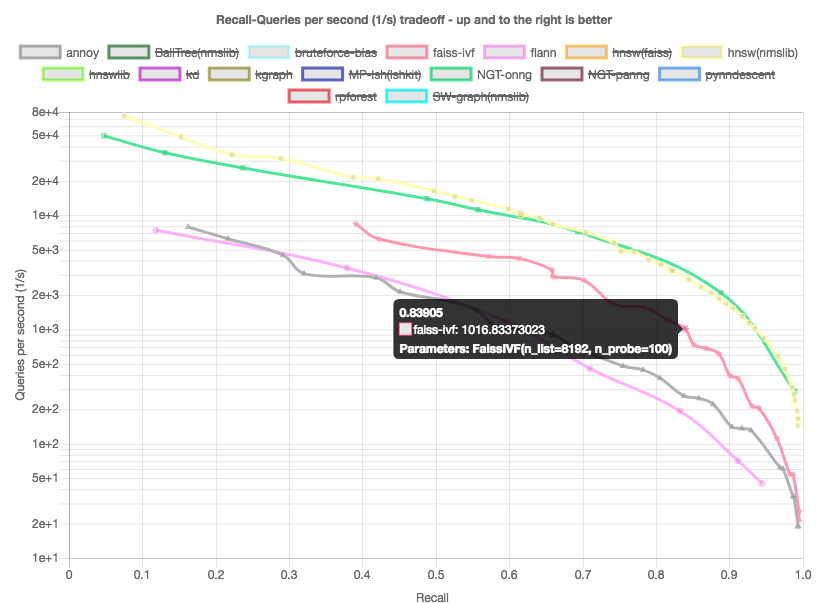
\includegraphics[width=0.9\textwidth]{figures/frontend-plot-uncropped}
\caption{Interactive plot screen from framework's website. 
Plot shows ``Queries per second'' ($y$-axis, log-scaled) against ``Recall'' ($x$-axis). 
Highlighted data point corresponds to a run of \textsf{FAISS-IVF} with parameters 
as depicted, giving about 1017 queries per second for a recall of about 0.84. The legend shows all available 
algorithm results; for the sake of presentation, results for the algorithms
with struck-out names are not included in the plot.}
\label{fig:interactive:plot}
\end{figure}

